\section{Observation and Calculations}

For normal Zeeman effect with transverse magnetic field, for different values of pole separation (i.e. different values of magnetic field), we have measured the radii of the spectral rings upto 3rd order.
\begin{table}[H]
    \centering
    \begin{tabular}{cccc}\hline
        \multicolumn{4}{c}{Radii ($\mu$m)}             \\\hline
        & $R_1$& $R_2$ & $R_3$  \\
        & (1st order)&(2nd order) & (3rd order) \\ \hline        
        \multicolumn{4}{l}{Pole separation = 40 mm}             \\\hline
        a &  30.54         &         139.47  &170.47           \\
        b &    72.16       &      140.53     &      180.27     \\
        c &       98.66    &159.69           &         188.19   \\\hline
        \multicolumn{4}{l}{Pole separation = 41 mm}             \\\hline
        a &    38.30       &128.51           &           168.97\\
        b &        71.16   &      139.47     &      180.44     \\
        c &      98.66     &           150.08&183.59            \\\hline
        \multicolumn{4}{l}{Pole separation = 42 mm}             \\ \hline
        a &   28.37        &   126.90        &168.48           \\
        b &    63.49       &    135.73        &     175.78      \\
        c &   85.02        &145.07           &182.98            \\\hline
        \multicolumn{4}{l}{Pole separation = 44 mm}             \\\hline
        a &  38.98         &          128.66 &168.82           \\
        b &      63.85     &      136.56     &      173.26     \\
        c &        82.02   & 143.55          &           178.39 \\\hline
        \multicolumn{4}{l}{Pole separation = 45 mm}             \\\hline
        a &  47.91         &         132.32  &173.78           \\
        b &      67.57     &    139.61       &     177.49      \\
        c &          82.58 &144.96           &          182.39  \\\hline
        \end{tabular}    
        \caption{Radii measured for each order for different values of pole separation. Here, Components of each order rings are designated as $a$, $b$ and $c$, where the outer $a$ and $c$ are $\sigma$ lines and the middle $b$ is $\pi$ line}
        \label{tab:1}
    \end{table}

Now, the average values of $\Delta$ and $\delta$ calculated from Table \ref{tab:1} using Eq. \ref{deltas} are outlined in Table \ref{tab:2}. These values are then used to measure the difference in wave number, $\Delta k$, using Eq. \ref{delk} (Table \ref{tab:3}).

\begin{table*}
    % \centering
\begin{ruledtabular}
    \begin{tabular}{cccccccccc}
             \multicolumn{5}{c}{$\delta_{n,xy}=R^2_{n,y}-R^2_{n,x}$ (mm$^2$)} &   \multicolumn{5}{c}{$\Delta^x_n=R^2_{n+1,x}-R^2_{n,x}$}  \\ \hline
             & $n=1$       & $n=2$       & $n=3$       &  Avg. ${\delta_{n,xy}}$  &                   & $x=a$        & $x=b$       & $x=c$       &  Avg. $\Delta^x_n$ \\ \hline
            \multicolumn{10}{l}{Pole separation = 40 mm}  \\ \hline
            $x=a$, $y=b$& 4274.37 & 3662.83 & 3437.25 & \multirow{2}{*}{4095.27} & $n=1$ & 15153.16 & 14541.62 & 15767.10 & \multirow{2}{*}{14236.93} \\
            $x=b$, $y=a$ & 4526.73 & 5752.22 & 2918.20 &  & $n=2$ & 12974.17 & 12478.59 & 9914.58 & \\
            \hline
            \multicolumn{10}{l}{Pole separation = 41 mm}  \\ \hline
            $x=a$, $y=b$& 3708.47 & 2937.06 & 4007.73 & \multirow{2}{*}{3071.92} & $n=1$ & 15047.93 & 14276.52 & 13789.24 & \multirow{2}{*}{13239.62} \\
            $x=b$, $y=a$ & 3559.41 & 3072.13 & 1146.69 &  & $n=2$ & 12036.04 & 13106.71 & 11181.28 & \\ \hline
            \multicolumn{10}{l}{Pole separation = 42 mm}  \\ \hline
            $x=a$, $y=b$& 3226.12 & 2319.02 & 2513.10 & \multirow{2}{*}{2743.57} & $n=1$ & 15298.75 & 14391.65 & 13816.91 & \multirow{2}{*}{13450.26} \\
            $x=b$, $y=a$ & 3197.42 & 2622.67 & 2583.07 &  & $n=2$ & 12281.90 & 12475.98 & 12436.38 & \\\hline
            \multicolumn{10}{l}{Pole separation = 44 mm}  \\ \hline
            $x=a$, $y=b$& 2557.38 & 2095.24 & 1518.84 & \multirow{2}{*}{2097.31} & $n=1$ & 15033.96 & 14571.81 & 13879.32 & \multirow{2}{*}{13003.11} \\
            $x=b$, $y=a$ & 2650.46 & 1957.97 & 1803.96 &  & $n=2$ & 11946.80 & 12011.75 & 9914.58 & \\ \hline
            \multicolumn{10}{l}{Pole separation = 45 mm}  \\ \hline
            $x=a$, $y=b$& 2270.34 & 1982.37 & 1303.21 & \multirow{2}{*}{1849.25} & $n=1$ & 15213.21 & 14925.25 & 14193.95 & \multirow{2}{*}{13547.96} \\
            $x=b$, $y=a$ & 2253.75 & 1522.45 & 1763.41 &  & $n=2$ & 12690.91 & 12011.75 & 12252.71 & \\
            \end{tabular}
        \caption{$\delta$ and $\Delta$ values calculated using Eq. \ref{deltas}. Here, $\delta$ is difference of squares of radii of different lines of same order, calculated for both the components of $\sigma$ line and take average. $\Delta$ is the difference of squares of radii of different order. Note that we have ignored the value of $\Delta^c_2$ in the avg. since it was too deviant from the other values.}
        \label{tab:2}
        \end{ruledtabular}
\end{table*}
\begin{table}[H]
    \centering
    \begin{tabular}{cccc} \hline
        Pole & $B$ & $\Delta k$ & $\mu_B$ \\ 
        Separation (mm) & (mT) & (m$^{-1}$) & ($\times 10^{-24}$ J/T) \\ \hline
        40 & 675 & 32.93 & 4.85 \\ 
        41 & 585 & 26.56 & 4.51 \\ 
        42 & 505 & 23.35 & 4.59 \\ 
        44 & 402 & 18.46 & 4.56 \\ 
        45 & 361 & 15.62 & 4.30 \\ \hline
    \end{tabular}    
        \caption{Values of pole separation and the corresponding values for $B$, $\Delta k$ and $\mu_B$}
        \label{tab:3}
    \end{table}

Rearranging Eq. \ref{straight}, we get 

\begin{align} \label{slope}
    \Delta k = \left(\frac{2\mu_B}{hc}\right)B
\end{align}

which is of the form $y=mx+b$. By performing a least square fit on the values of Table \ref{tab:3} shown in Fig. \ref{plot}, we get the slope, $m=52.503 \text{ m}^{-1} \text{ T}^{-1}$ which translates to $\mu_B=5.215 \times 10^{-24}$ J/T.

\begin{figure}
    \centering
    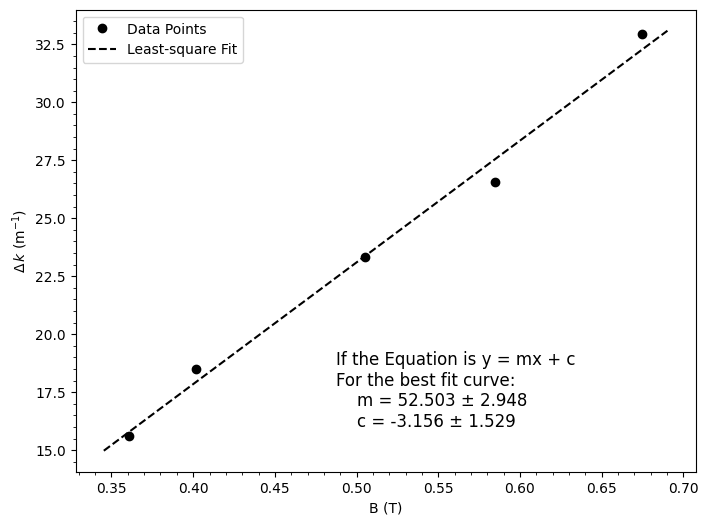
\includegraphics[width=1\columnwidth]{images/plot.png}
    \caption{Least-square fitting for the $\Delta k$ vs. $B$ plot}
    \label{plot}
\end{figure}

\begin{figure*}
    \centering
    \begin{subfigure}[b]{0.45\textwidth}
        \centering
        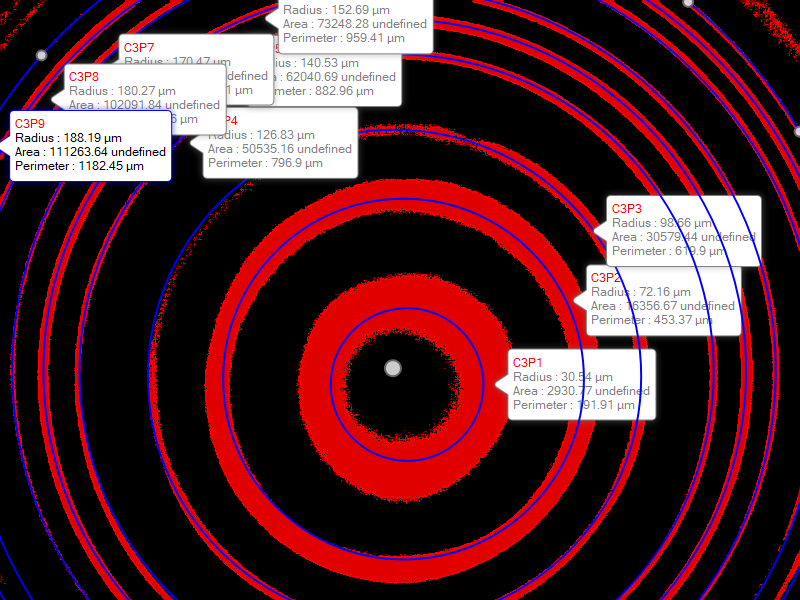
\includegraphics[width=\textwidth]{images/40.png}
        \caption{$d=40$ mm}
    \end{subfigure}
    \hfill
    \begin{subfigure}[b]{0.45\textwidth}
        \centering
        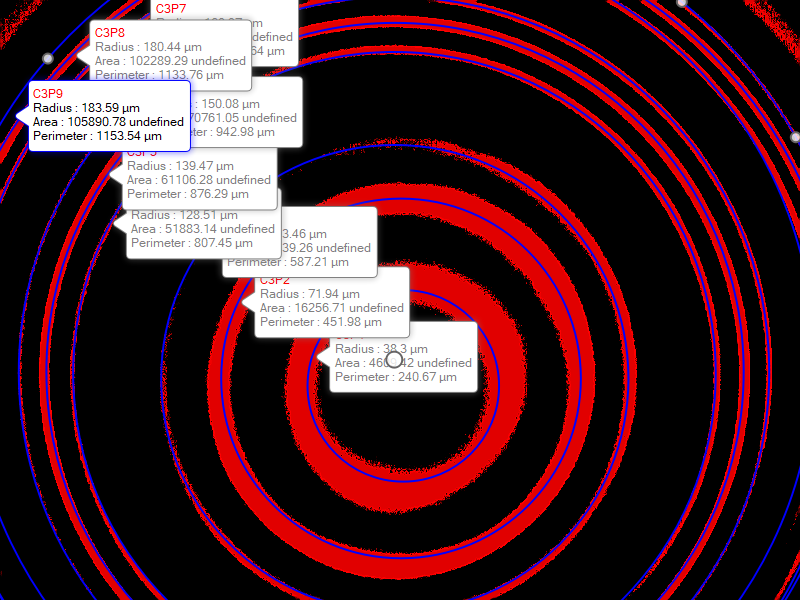
\includegraphics[width=\textwidth]{images/41.png}
        \caption{$d=41$ mm}
    \end{subfigure}
    \hfill
    \begin{subfigure}[b]{0.45\textwidth}
        \centering
        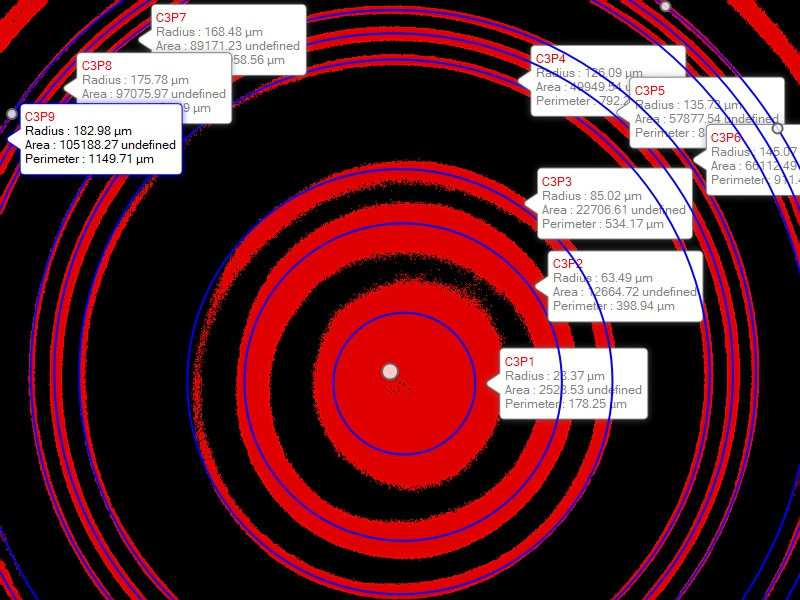
\includegraphics[width=\textwidth]{images/42.jpg}
        \caption{$d=42$ mm}
    \end{subfigure}
    \hfill
    \begin{subfigure}[b]{0.45\textwidth}
        \centering
        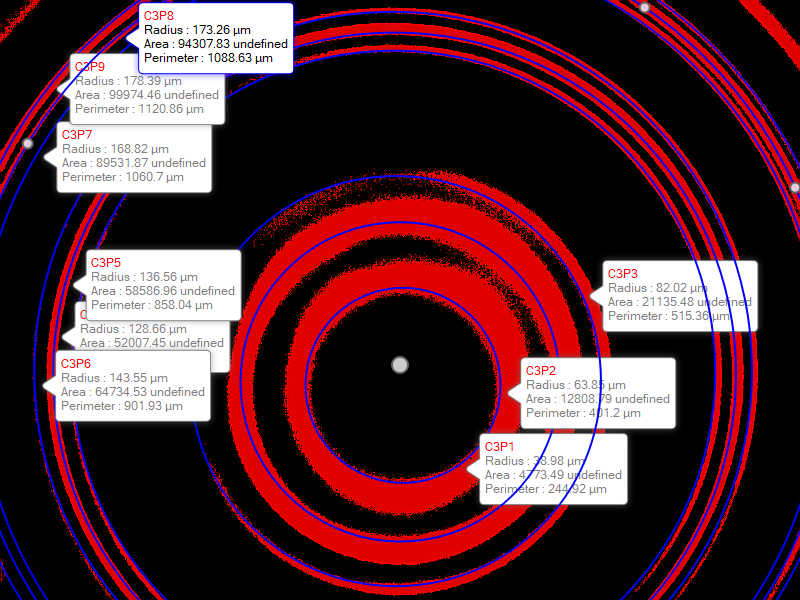
\includegraphics[width=\textwidth]{images/44.png}
        \caption{$d=44$ mm}
    \end{subfigure}
    \hfill
    \begin{subfigure}[b]{0.45\textwidth}
        \centering
        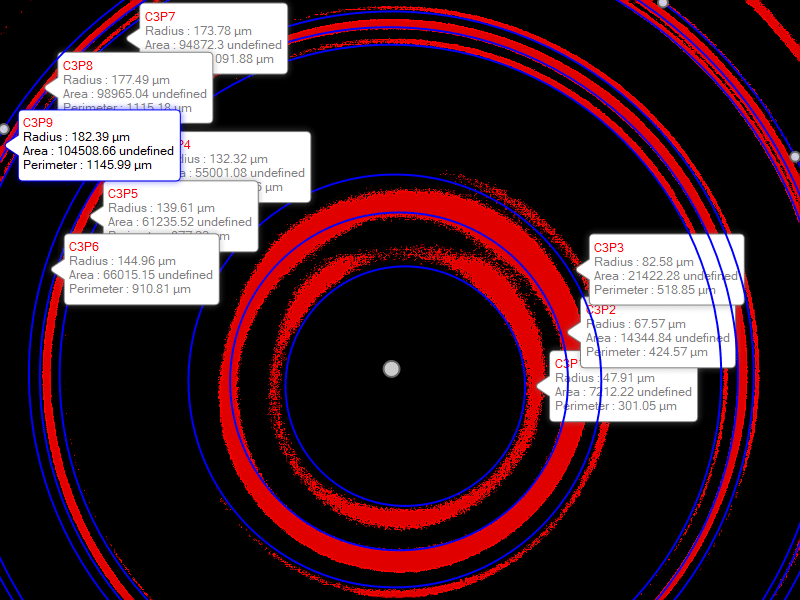
\includegraphics[width=\textwidth]{images/45.png}
        \caption{$d=45$ mm}
    \end{subfigure}
    \hfill
    \caption{Normal Zeeman effect observed for different values of magnetic field, i.e. pole separation ($d$)}\label{f1}
\end{figure*}

\begin{figure*}
    \centering
    \begin{subfigure}[b]{0.45\textwidth}
        \centering
        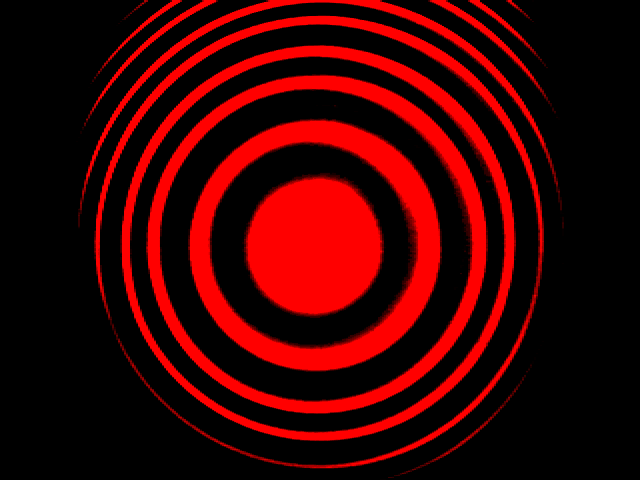
\includegraphics[width=\textwidth]{images/longitudinal_no_polarizer.png}
        \caption{Without any polarization filter}
    \end{subfigure}
    \hfill
    \begin{subfigure}[b]{0.45\textwidth}
        \centering
        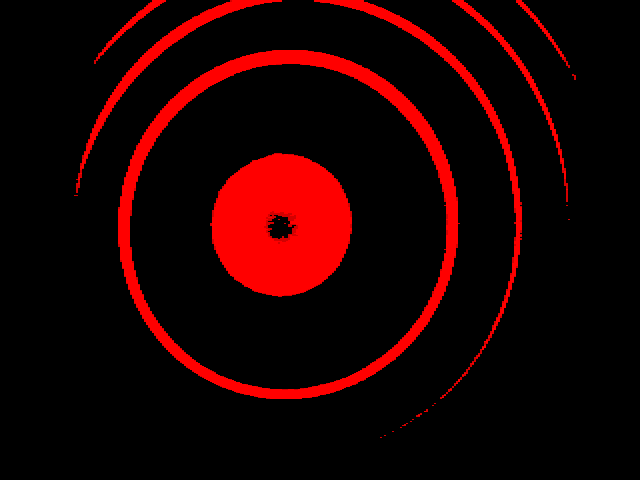
\includegraphics[width=\textwidth]{images/left.png}
        \caption{Left circularly polarized light}
    \end{subfigure}
    \hfill
    \begin{subfigure}[b]{0.45\textwidth}
        \centering
        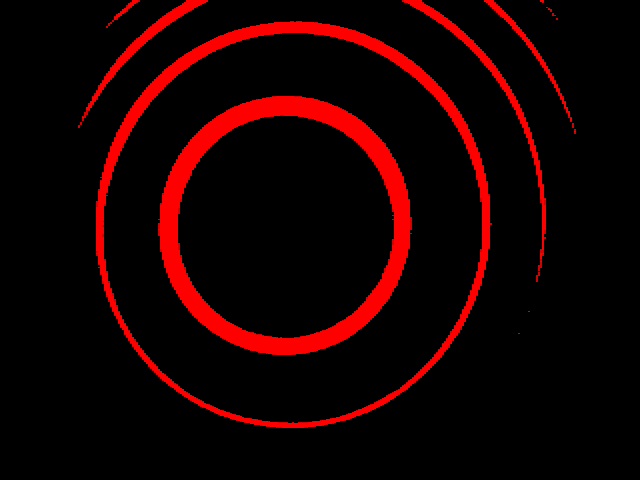
\includegraphics[width=\textwidth]{images/right_correct.png}
        \caption{Right circularly polarized light}
    \end{subfigure}
    \caption{Normal Zeeman Effect observed with longitudinal magnetic field}\label{f2}
\end{figure*}

\begin{figure*}
    \centering
    \begin{subfigure}[b]{0.45\textwidth}
        \centering
        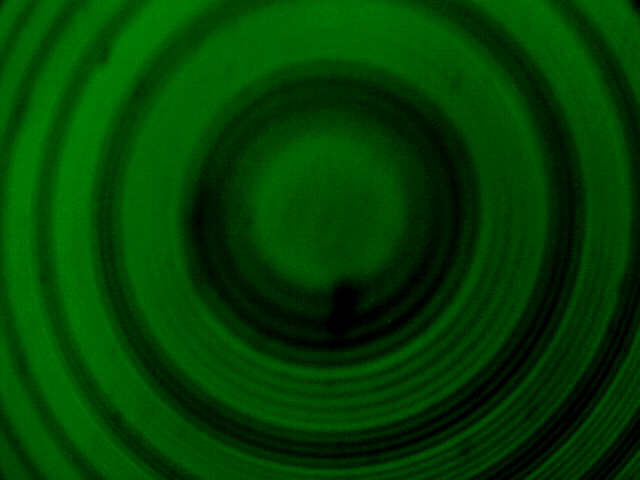
\includegraphics[width=\textwidth]{images/ano4.png}
        \caption{Without any polarization filter}
    \end{subfigure}
    \hfill
    \begin{subfigure}[b]{0.45\textwidth}
        \centering
        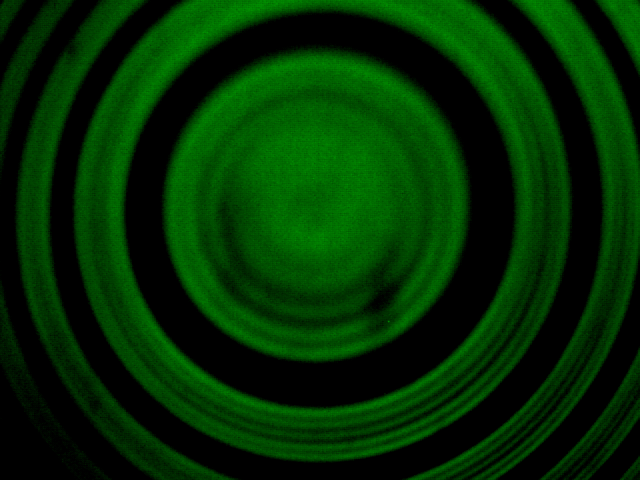
\includegraphics[width=\textwidth]{images/sigma.png}
        \caption{$\sigma$ lines observed}
    \end{subfigure}
    \hfill
    \begin{subfigure}[b]{0.45\textwidth}
        \centering
        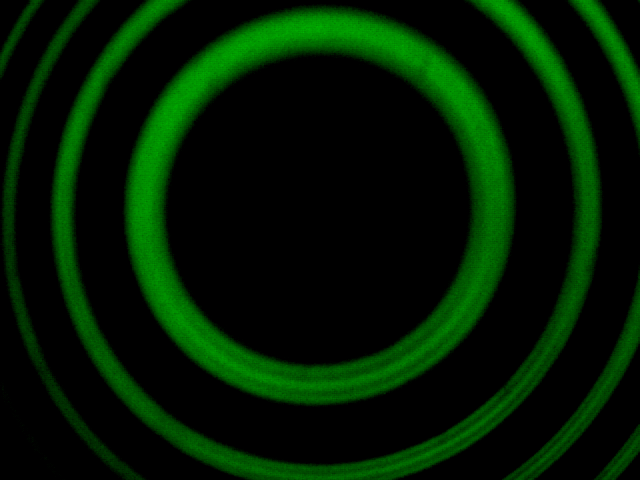
\includegraphics[width=\textwidth]{images/pi.png}
        \caption{$\pi$ lines observed}
    \end{subfigure}\hfill
    \begin{subfigure}[b]{0.45\textwidth}
        \centering
        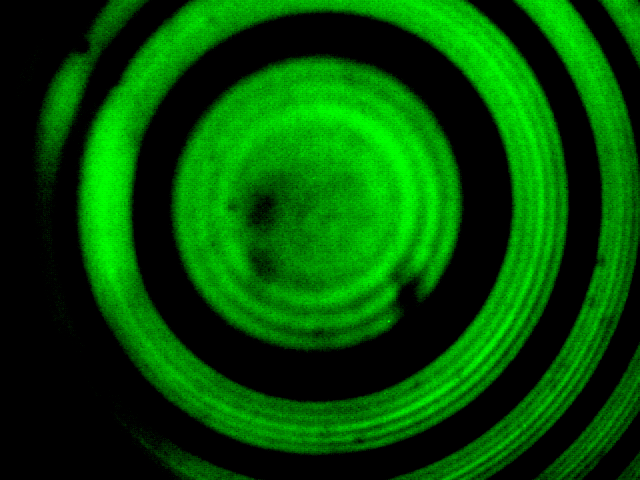
\includegraphics[width=\textwidth]{images/anomalous_longitudinal.png}
        \caption{Only sigma lines observed even without the polarization filter in case of longitudinal magnetic field}
        \label{ano_long}
    \end{subfigure}
    \caption{Anomalous Zeeman Effect observed in (a) to (c) transverse and (d) longitudinal magnetic fields}\label{f3}
\end{figure*}
The rest of the observations for normal and anomalous Zeeman effect are provided at the end (Figs. \ref{f2}, \ref{f3})

\subsection*{Error Analysis}
Using Eq. \ref{slope}, we can write the uncertainity in $\mu_B$ as,

\begin{align}
    \frac{\Delta \mu_B}{\mu_B} =  \frac{\Delta m}{m}
\end{align}

where $m$ is the slope. Hence, we get

\begin{align*}
    \Delta \mu_B = \frac{5.215 \times 10^{-24} \times 2.948}{52.503} = 0.293 \times 10^{-24} \text{ J/T}
\end{align*}
